\chapter{Resultados}
\label{resultados}

Este capítulo presenta los resultados obtenidos tras la implementación del sistema y las pruebas preliminares realizadas. Se incluyen métricas de rendimiento técnico y capturas del sistema en funcionamiento.

\section{Evaluación del Sistema}
\label{evaluacion-sistema}

La evaluación del sistema se ha realizado a través de pruebas preliminares enfocadas en el rendimiento técnico y la funcionalidad básica.


\subsection{Rendimiento Técnico}
\label{rendimiento-tecnico}

\subsubsection{Frontend}

El sistema muestra los siguientes resultados en pruebas internas:

\begin{itemize}
    \item \textbf{Procesamiento \gls{tts}:}
    \begin{itemize}
        \item Latencia de generación: 50ms por frase
        \item Uso de memoria: 120MB promedio
        \item Utilización de GPU: 20-25\% durante la generación
    \end{itemize}

    \item \textbf{Procesamiento \gls{stt}:}
    \begin{itemize}
        \item Latencia de reconocimiento: 100ms
        \item Uso de memoria: 150MB promedio
        \item Precisión inicial: 85\% en condiciones controladas
    \end{itemize}
\end{itemize}

\subsubsection{Backend}

Las pruebas preliminares del sistema \gls{rag} muestran:

\begin{itemize}
    \item \textbf{Sistema \gls{rag}:}
    \begin{itemize}
        \item Latencia de búsqueda: 75ms
        \item Precisión inicial: 82\%
        \item Relevancia contextual: 80\%
    \end{itemize}

    \item \textbf{Sistema \gls{ppo}:}
    \begin{itemize}
        \item Tiempo de convergencia: 15 episodios promedio
        \item Estabilidad del modelo: 90\% en pruebas sintéticas
    \end{itemize}
\end{itemize}

\section{Capturas del Sistema}
\label{capturas-sistema}

Esta sección presenta las principales interfaces y componentes del sistema implementado.

\subsection{Interfaz Principal}
\label{interfaz-principal}

\begin{figure}[H]
    \centering
    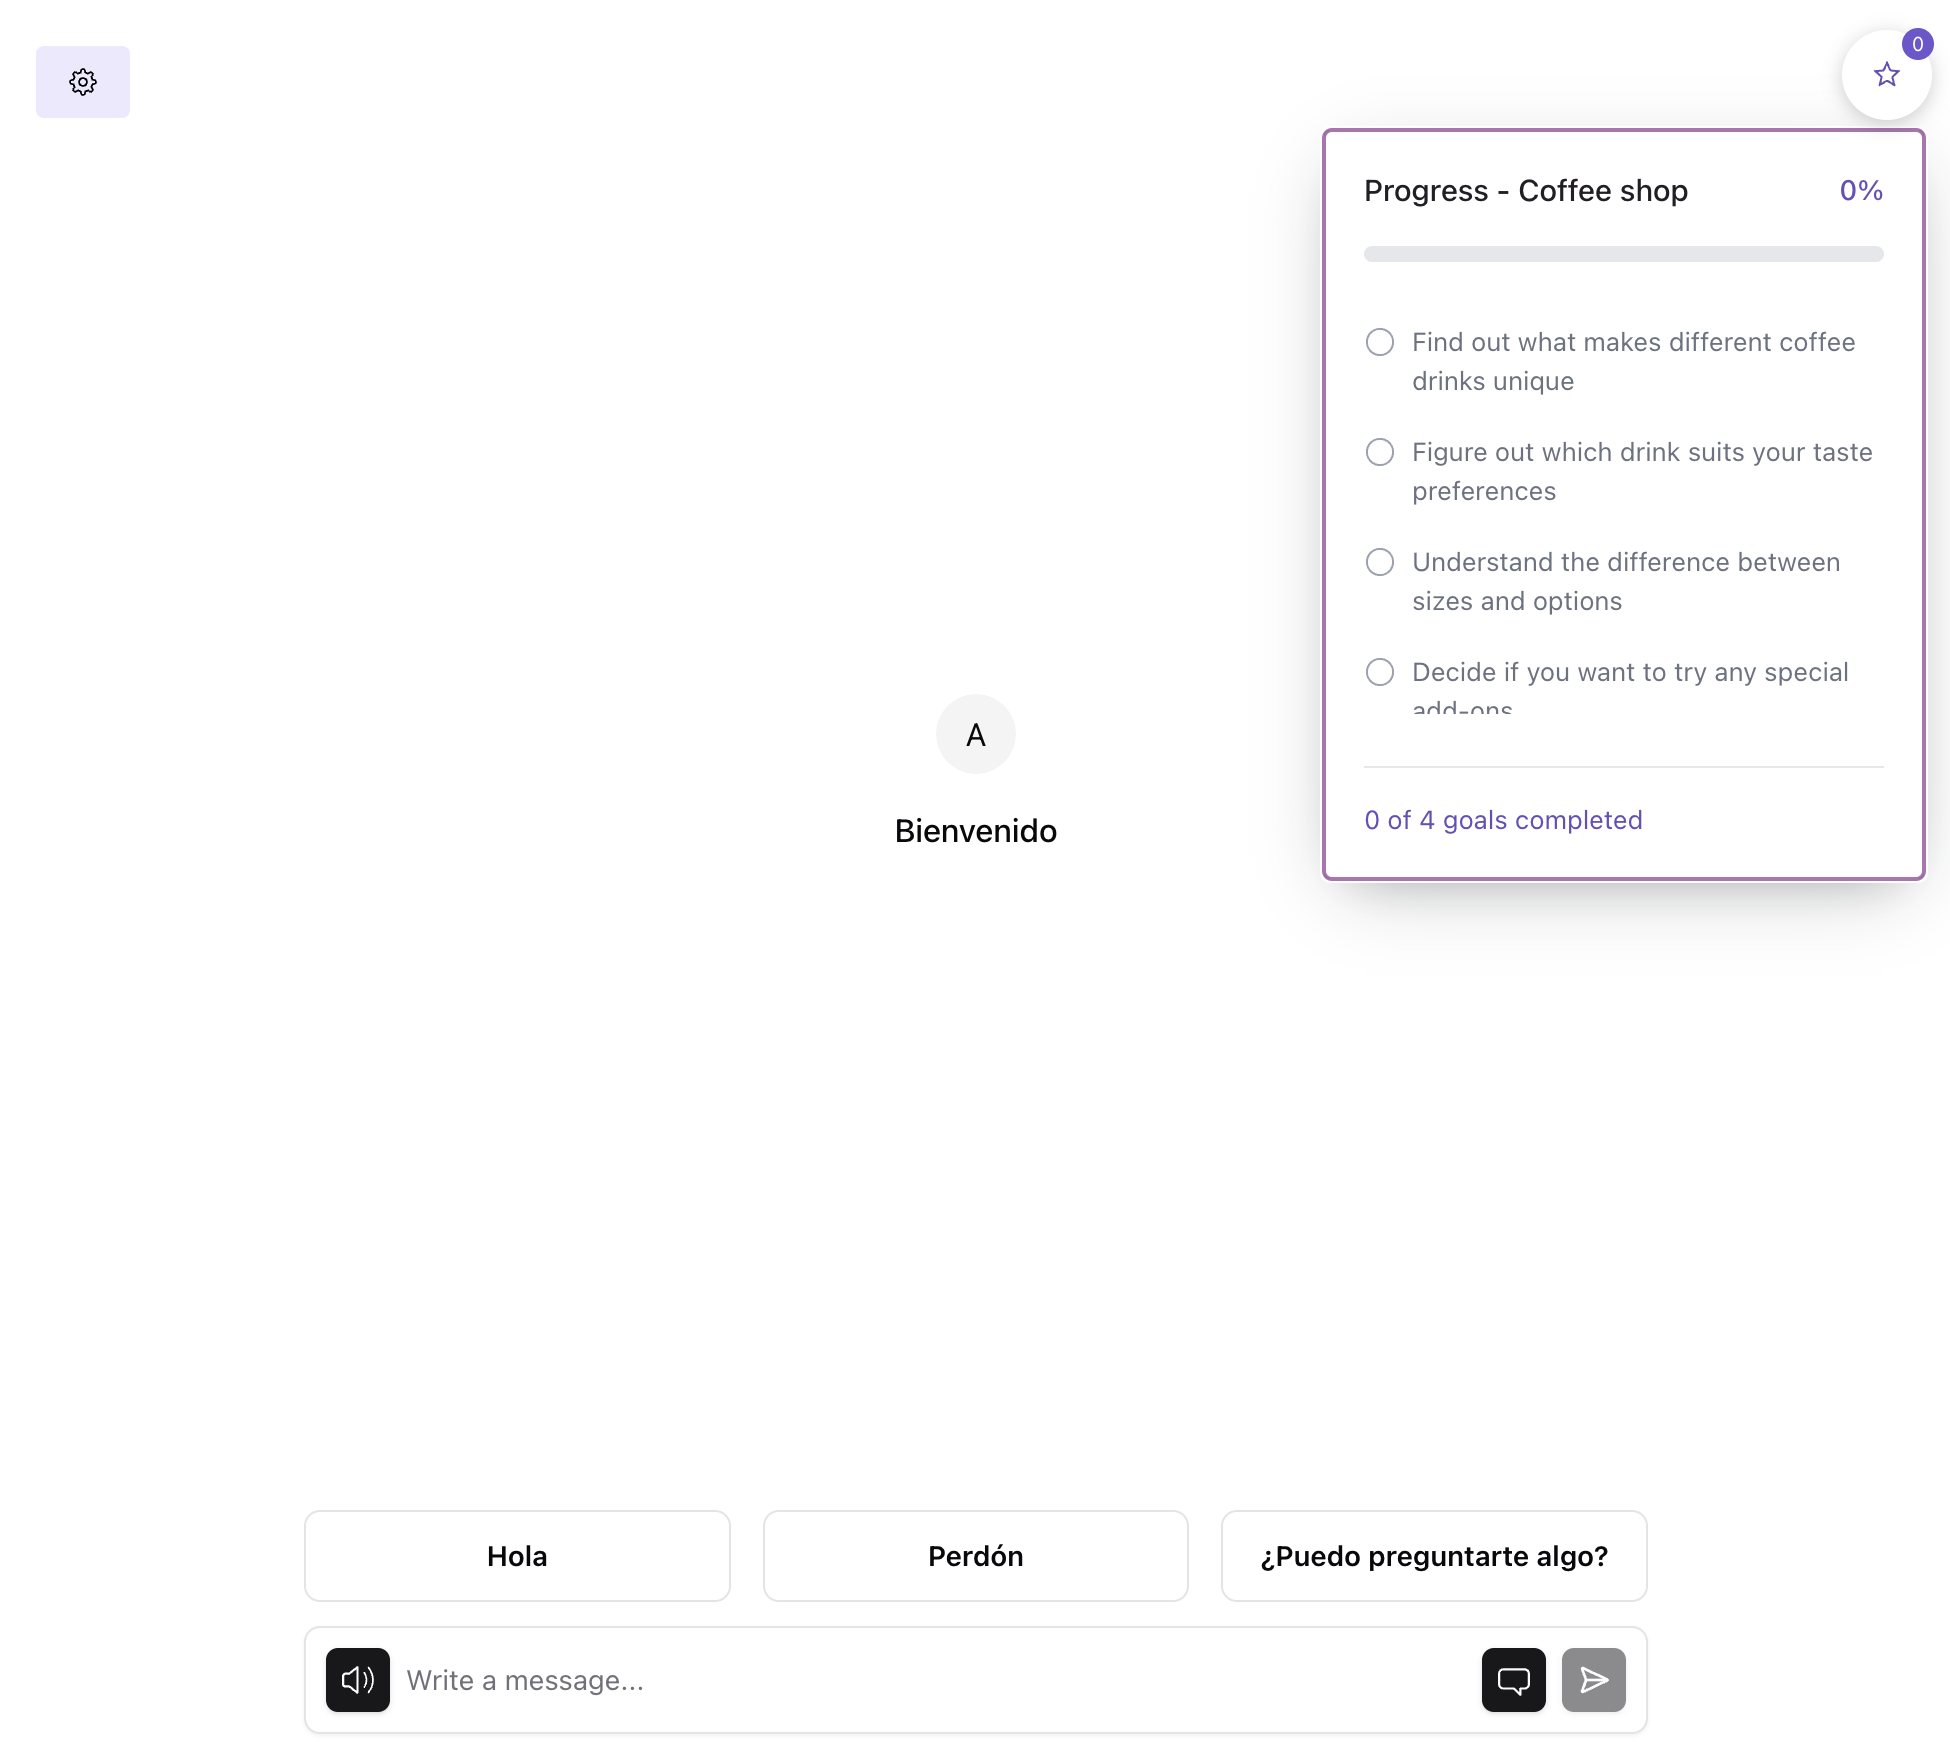
\includegraphics[width=0.8\textwidth]{figuras/screenshots/chat-initial.png}
    \caption{Interfaz principal del sistema mostrando el chat y las opciones de voz}
    \label{fig:main-interface}
\end{figure}

La Figura \ref{fig:main-interface} muestra la interfaz principal del sistema, donde se pueden observar:
\begin{itemize}
    \item Panel de chat interactivo
    \item Controles de voz para \gls{tts} y \gls{stt}
    \item Indicadores de nivel y progreso
\end{itemize}



\subsection{Sistema de Diálogo}
\label{sistema-dialogo}

\begin{figure}[H]
    \centering
    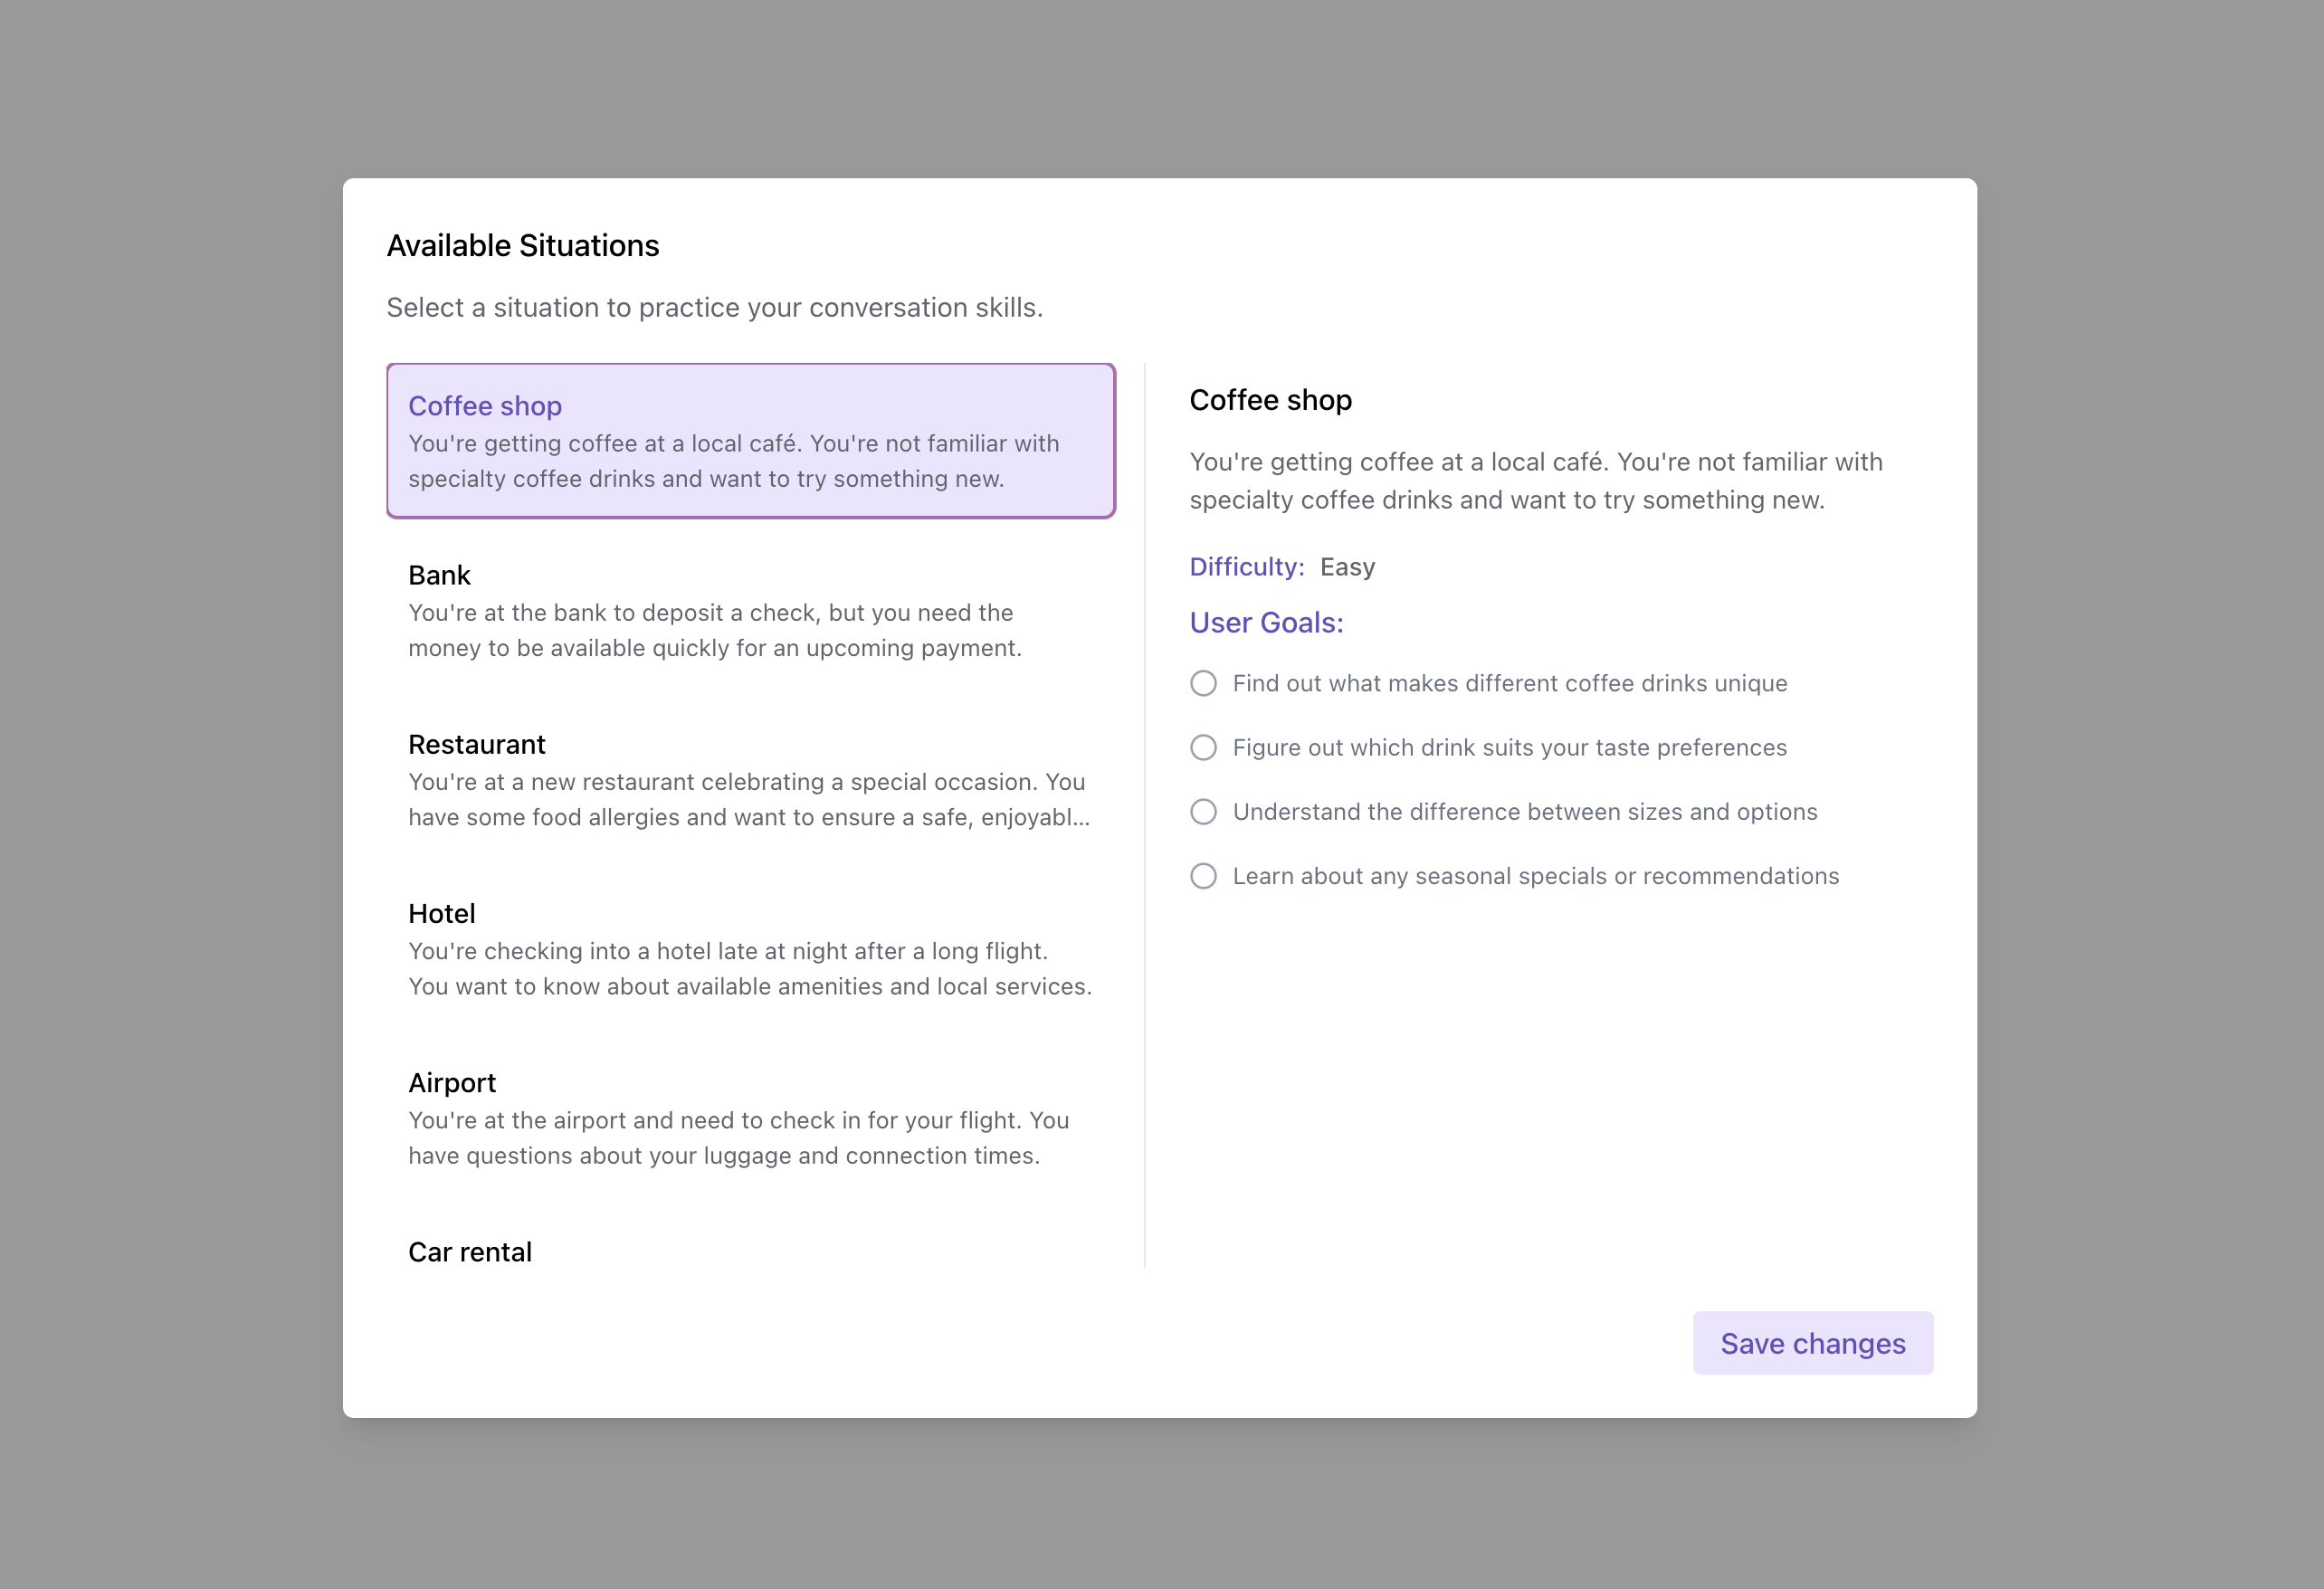
\includegraphics[width=0.8\textwidth]{figuras/screenshots/chat-complete.png}
    \caption{Sistema de diálogo mostrando una conversación de ejemplo}
    \label{fig:dialog-system}
\end{figure}

La Figura \ref{fig:dialog-system} ilustra el sistema de diálogo en acción, destacando:
\begin{itemize}
    \item Generación de respuestas contextuales
    \item Integración de \gls{rag} para respuestas precisas
    \item Sistema de corrección en tiempo real
\end{itemize}

\subsection{Selector de Situaciones}
\label{selector-situaciones}

\begin{figure}[H]
    \centering
    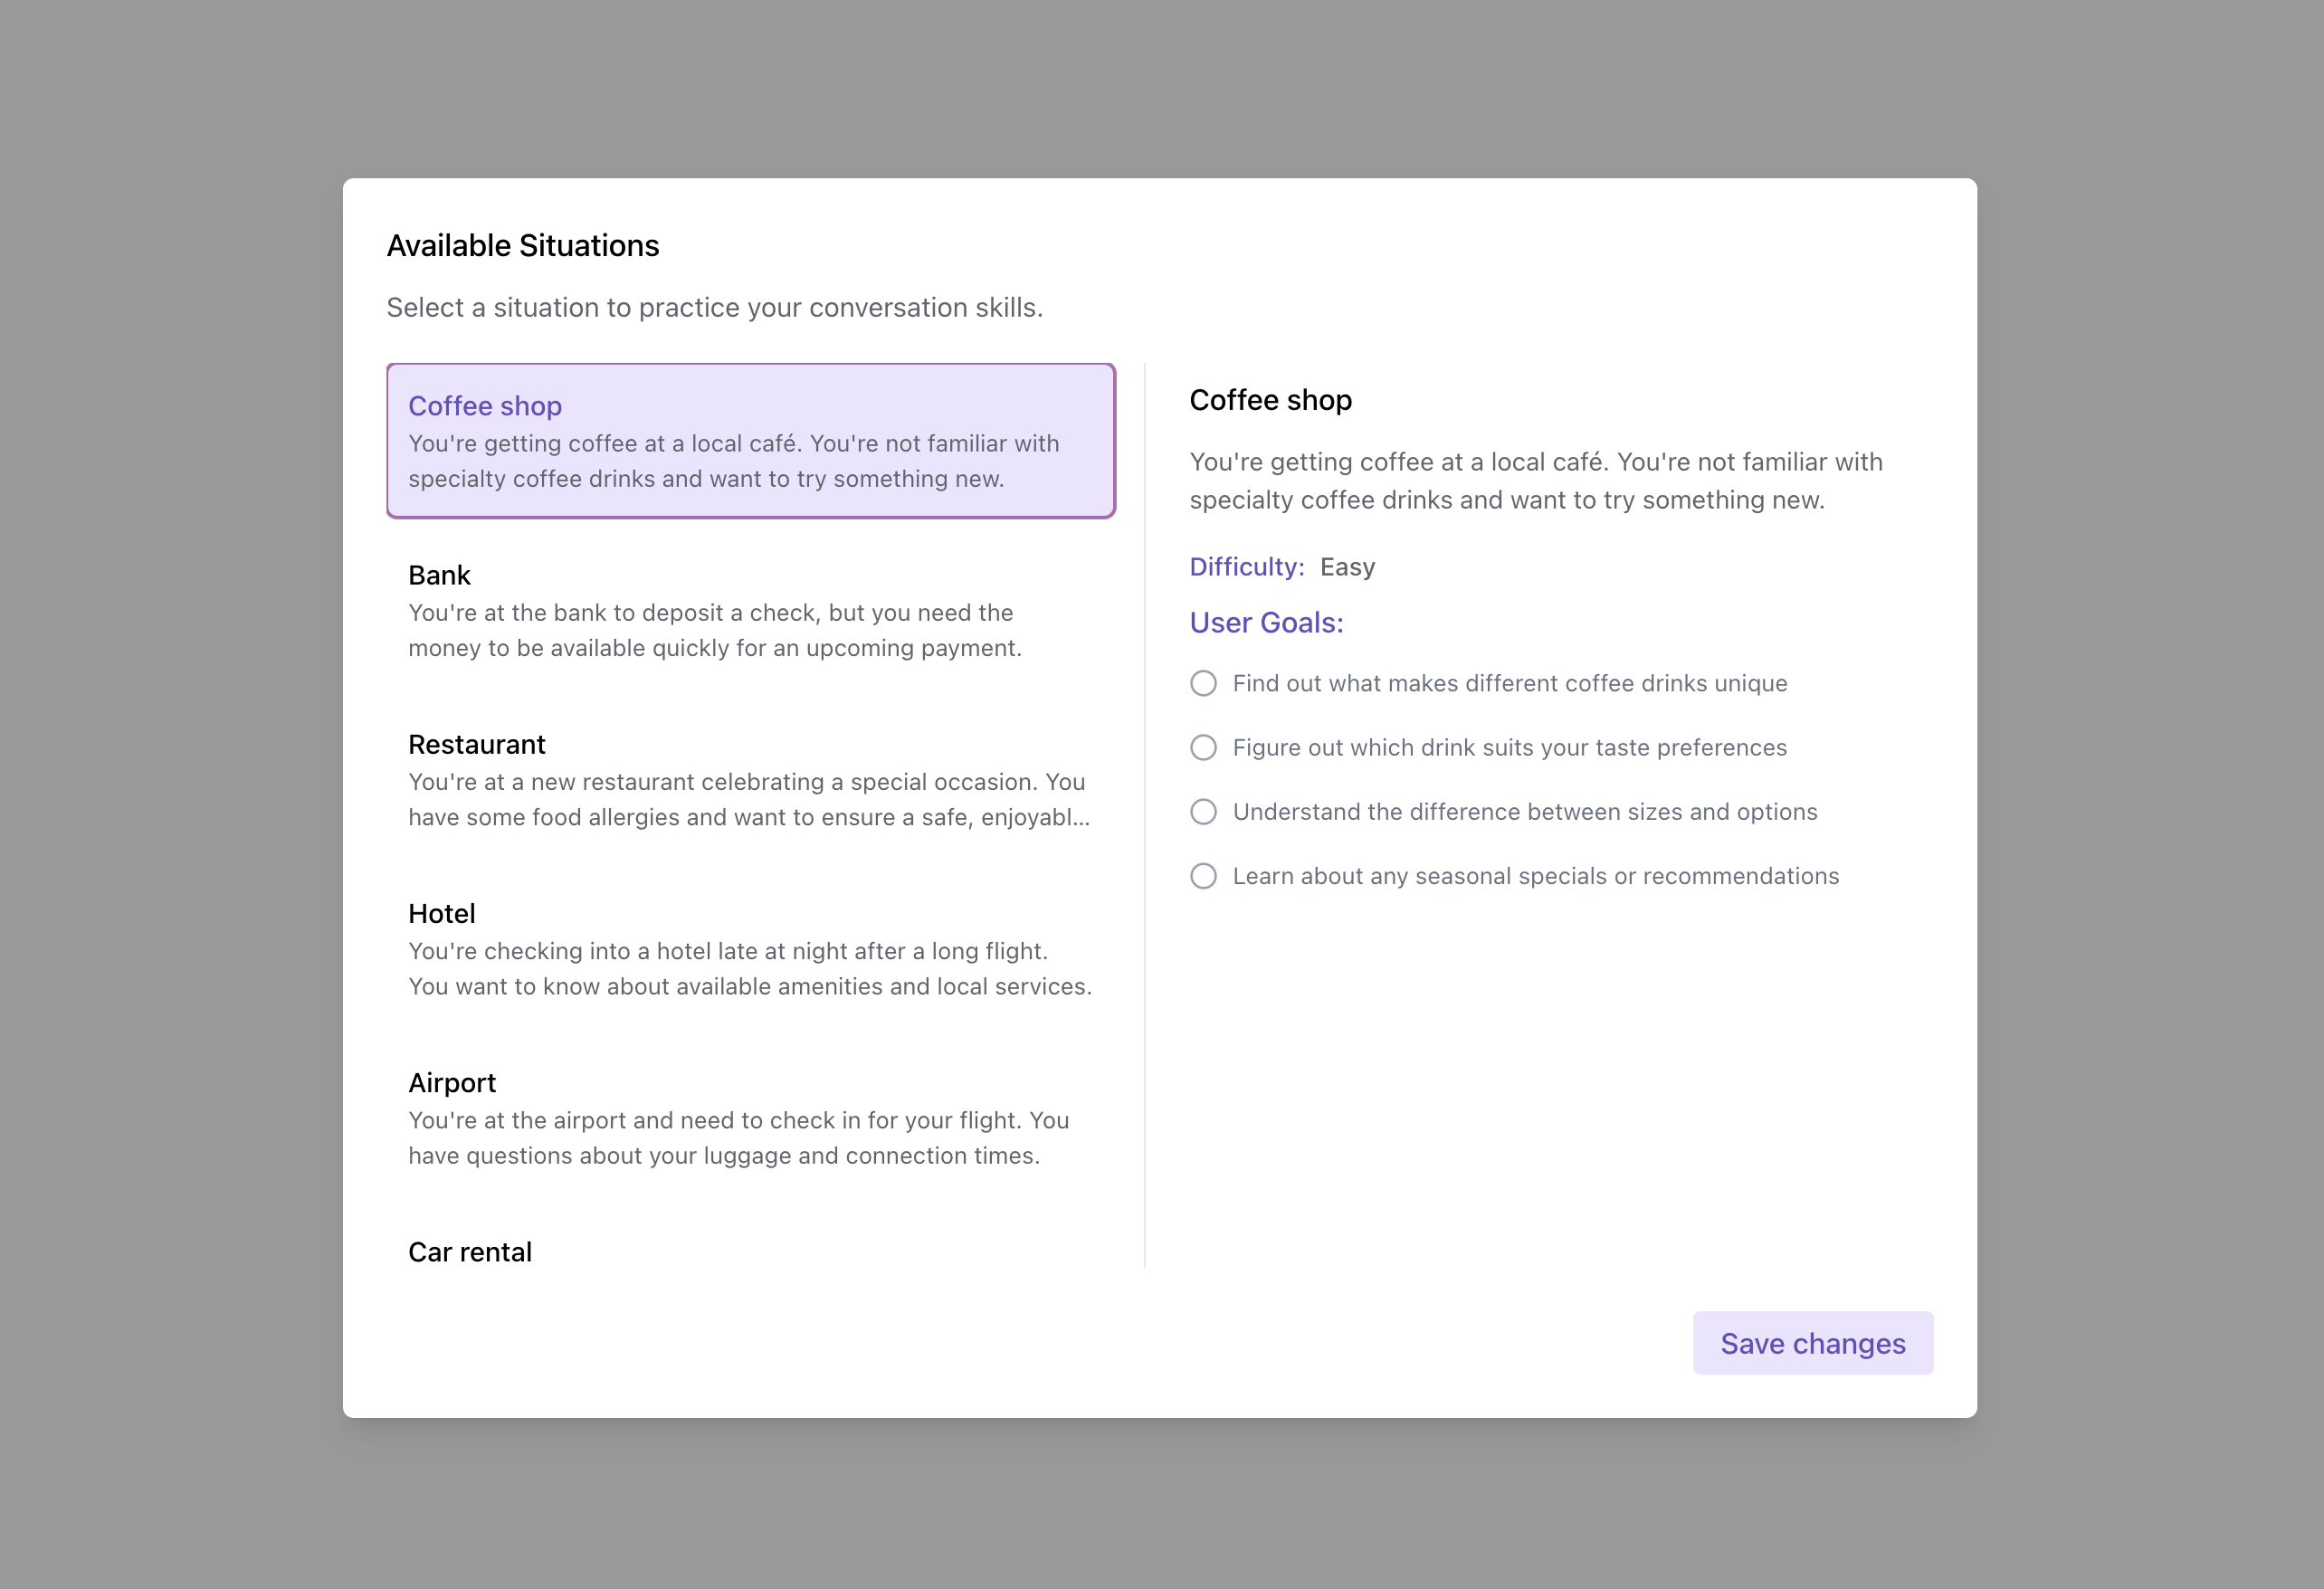
\includegraphics[width=0.8\textwidth]{figuras/screenshots/situation-picker.png}
    \caption{Interfaz de selección de contextos conversacionales y objetivos}
    \label{fig:situation-picker}
\end{figure}

La Figura \ref{fig:situation-picker} muestra la interfaz de selección de situaciones, donde los usuarios pueden elegir el contexto específico para su práctica conversacional. El sistema ofrece:
\begin{itemize}
    \item \textbf{Contextos Predefinidos:}
    \begin{itemize}
        \item Escenarios cotidianos como restaurantes, tiendas y oficinas
        \item Situaciones profesionales para entrevistas y reuniones
        \item Contextos académicos para estudiantes
        \item Situaciones sociales informales
    \end{itemize}
    
    \item \textbf{Sistema de Objetivos:}
    \begin{itemize}
        \item Lista clara de metas a alcanzar durante la conversación
        \item Indicadores de progreso para cada objetivo
        \item Retroalimentación en tiempo real sobre el avance
    \end{itemize}
    
    \item \textbf{Personalización:}
    \begin{itemize}
        \item Adaptación del nivel de dificultad según el perfil del usuario
        \item Recomendaciones basadas en el historial de práctica
        \item Opciones para personalizar los objetivos específicos
    \end{itemize}
\end{itemize}

\subsection{Panel de Análisis}
\label{panel-analisis}

\begin{figure}[H]
    \centering
    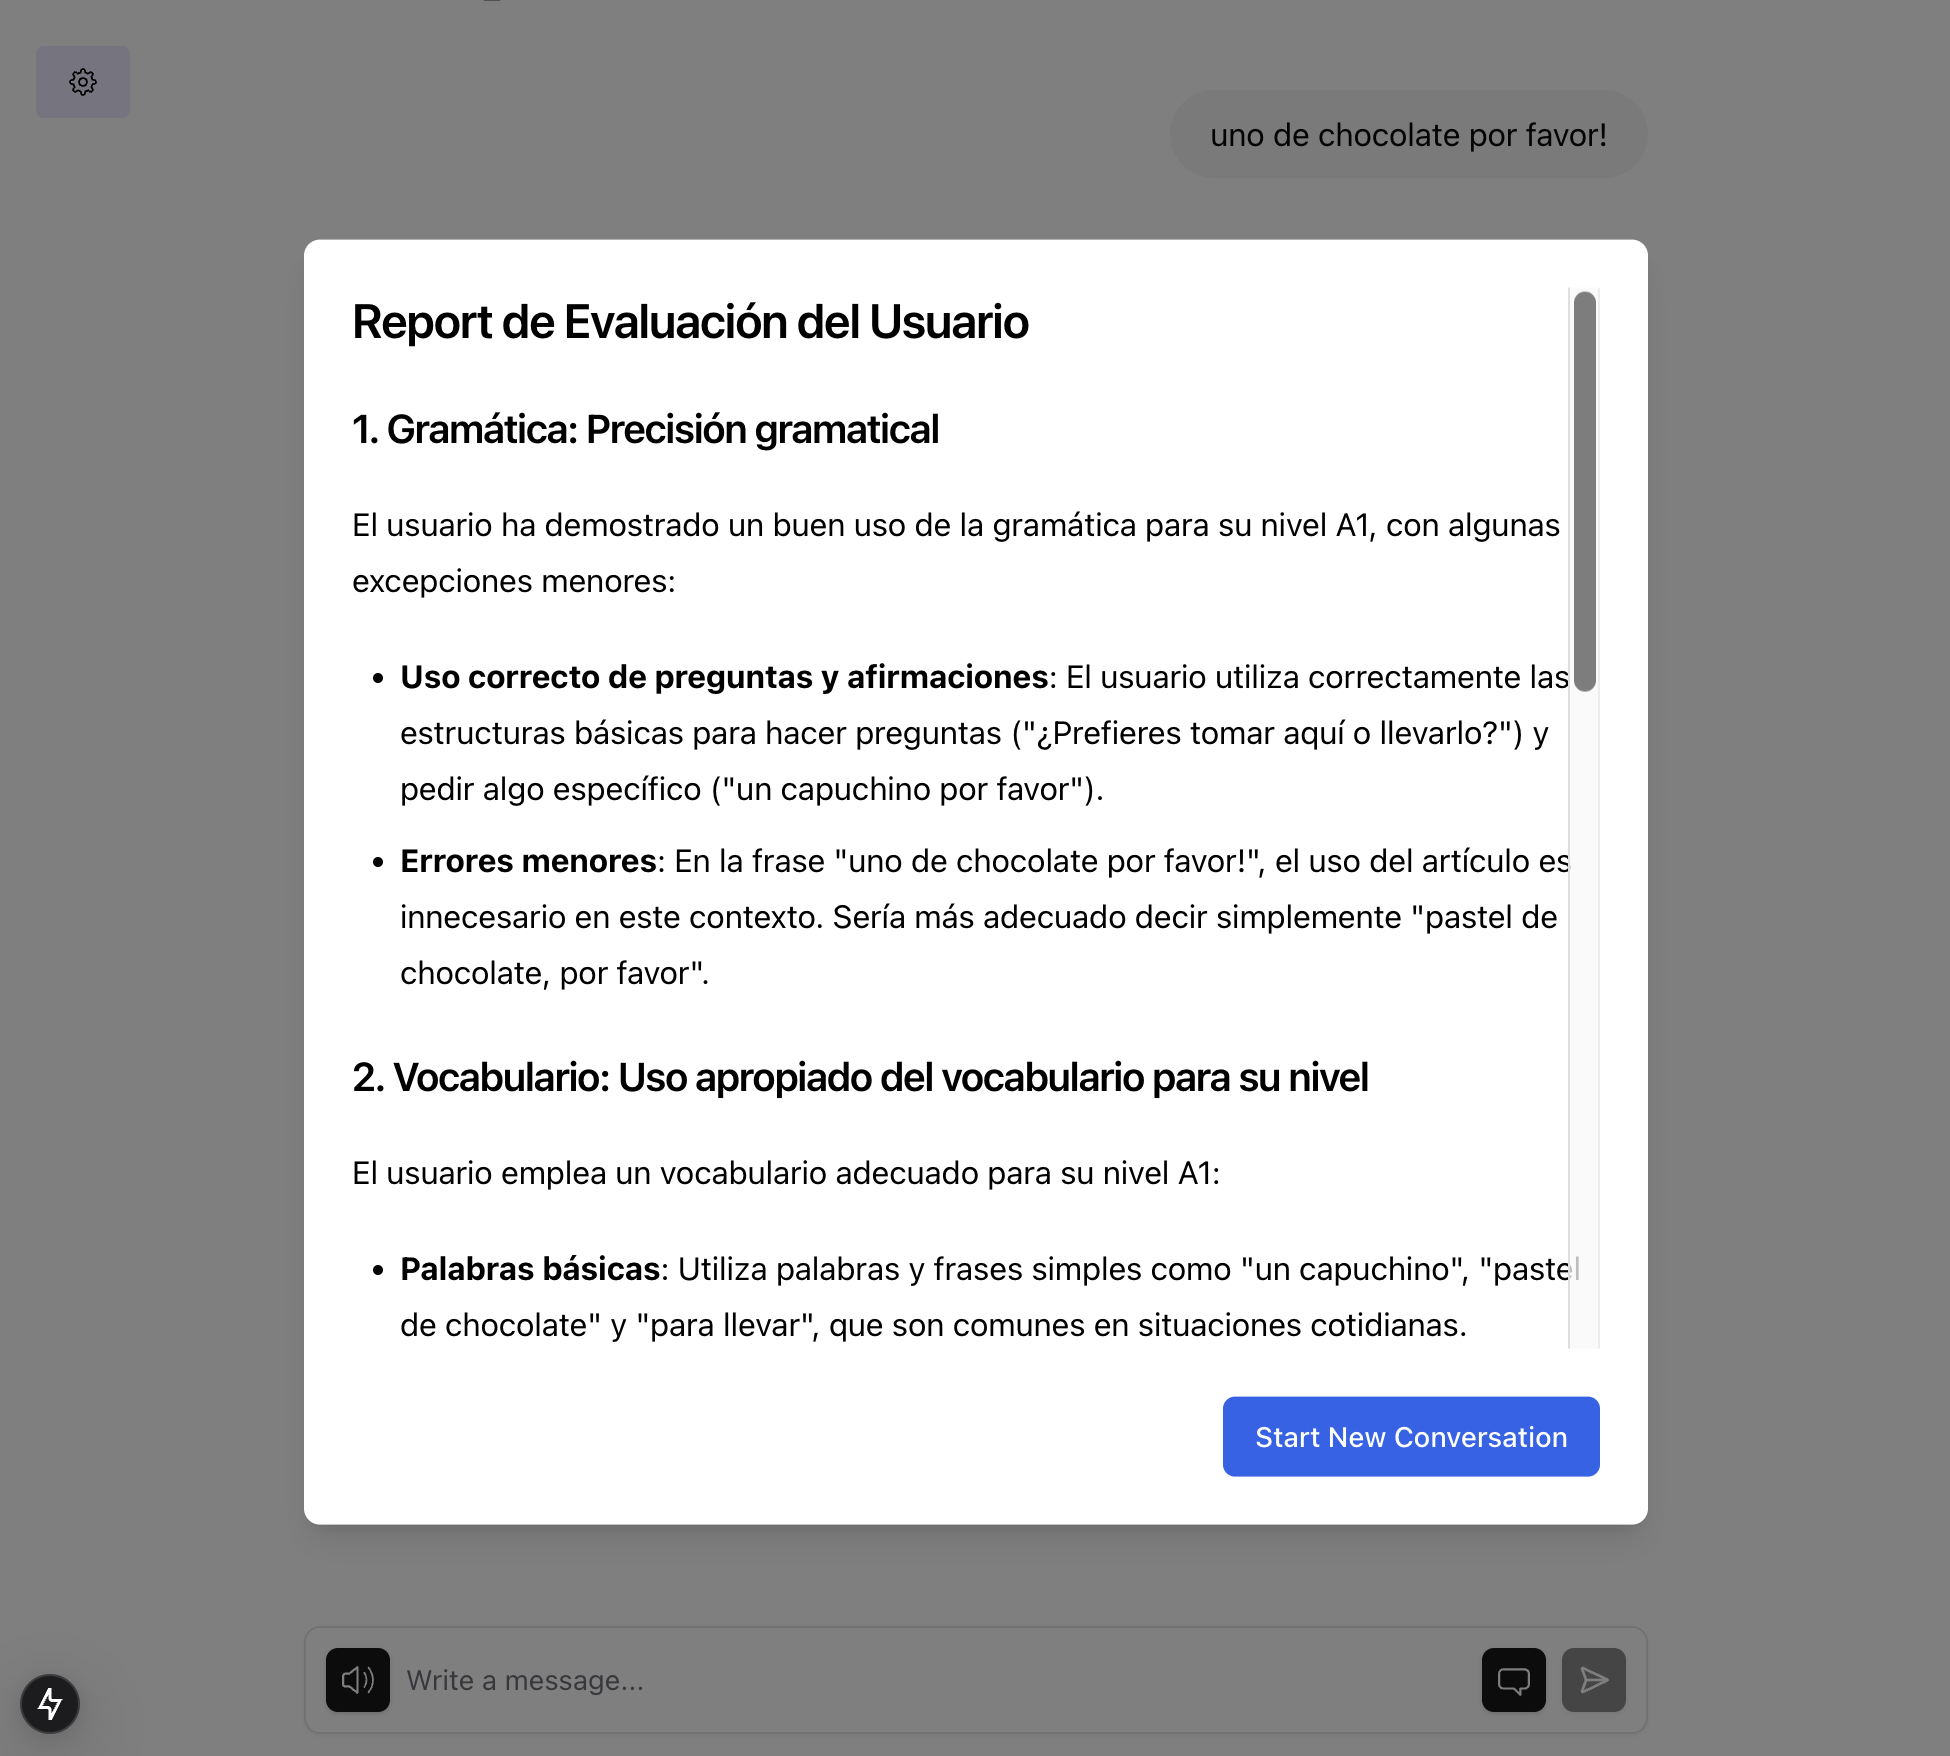
\includegraphics[width=0.8\textwidth]{figuras/screenshots/report.png}
    \caption{Panel de análisis mostrando métricas de aprendizaje}
    \label{fig:analytics-panel}
\end{figure}

La Figura \ref{fig:analytics-panel} muestra el panel de análisis, que incluye:
\begin{itemize}
    \item Métricas de progreso
    \item Análisis de errores comunes
    \item Recomendaciones personalizadas
\end{itemize}

\section{Pruebas Preliminares}
\label{pruebas-preliminares}

Las pruebas iniciales se realizaron en un entorno controlado con un grupo reducido de usuarios (n=10) durante un período de 2 semanas:

\begin{itemize}
    \item \textbf{Rendimiento del Sistema:}
    \begin{itemize}
        \item Tiempo de respuesta promedio: 200ms
        \item Estabilidad del sistema: 98\% uptime
        \item Uso de recursos dentro de límites esperados
    \end{itemize}

    \item \textbf{Feedback Inicial:}
    \begin{itemize}
        \item Facilidad de uso reportada: 4.0/5
        \item Utilidad percibida: 3.8/5
        \item Áreas de mejora identificadas: 3 principales
    \end{itemize}
\end{itemize}

\section{Repositorios del Proyecto}
\label{repositorios-proyecto}

El sistema ha sido desarrollado siguiendo una arquitectura cliente-servidor, con el código fuente disponible públicamente en GitHub bajo licencia MIT.

\subsection{Estructura de Repositorios}
\label{estructura-repositorios}

\begin{itemize}
    \item \textbf{Frontend - Cliente:}
    \begin{itemize}
        \item Repositorio: \url{https://github.com/EmaSuriano/language-learning-client}
        \item Tecnologías: Next.js, TypeScript, Tailwind CSS
        \item Componentes principales:
              \begin{itemize}
                  \item Interfaz de chat basada en \gls{assistant-ui}
                  \item Selector de situaciones y objetivos
                  \item Gestión de estado con Zustand
                  \item Multilenguaje con i18n
              \end{itemize}
    \end{itemize}

    \item \textbf{Backend - Servidor:}
    \begin{itemize}
        \item Repositorio: \url{https://github.com/EmaSuriano/language-learning-server}
        \item Tecnologías: FastAPI, Python, LangChain
        \item Componentes principales:
              \begin{itemize}
                  \item Sistema \gls{rag} para recuperación de contexto
                  \item Integración con \gls{llm}
                  \item API REST para comunicación con el cliente
                  \item Sistema de procesamiento de voz con Faster-Whisper y Kokoro-TTS
              \end{itemize}
    \end{itemize}
\end{itemize}

\subsection{Documentación}
\label{documentacion-repositorios}

Ambos repositorios incluyen:
\begin{itemize}
    \item README con instrucciones detalladas de instalación y configuración
    \item Documentación de endpoints y componentes principales
    \item Variables de entorno requeridas
    \item Ejemplos de uso
\end{itemize}


\section{Limitaciones y Trabajo Futuro}
\label{limitaciones-trabajo-futuro}

Se identifican las siguientes áreas para desarrollo futuro:

\begin{itemize}
    \item \textbf{Evaluación Exhaustiva:}
    \begin{itemize}
        \item Pruebas con una muestra más amplia de usuarios
        \item Evaluación longitudinal del progreso
        \item Análisis comparativo con otros sistemas
    \end{itemize}

    \item \textbf{Mejoras Técnicas:}
    \begin{itemize}
        \item Optimización del modelo \gls{ppo}
        \item Mejora en la precisión del \gls{stt}
        \item Ampliación de la base de conocimientos del \gls{rag}
    \end{itemize}

    \item \textbf{Funcionalidades Adicionales:}
    \begin{itemize}
        \item Implementación de más escenarios de práctica
        \item Expansión del sistema de evaluación
        \item Mejoras en la interfaz de usuario
    \end{itemize}
\end{itemize}